
\section{Introduction}


\begin{frame}
\frametitle{Initial Overview}

\begin{itemize}[<+->]
  \item The B method supports the construction of safety systems
  \begin{itemize}
    \item Until the implementation model
    \item But the result of this translation is not guaranteed by formal means\\
    \begin{center}
       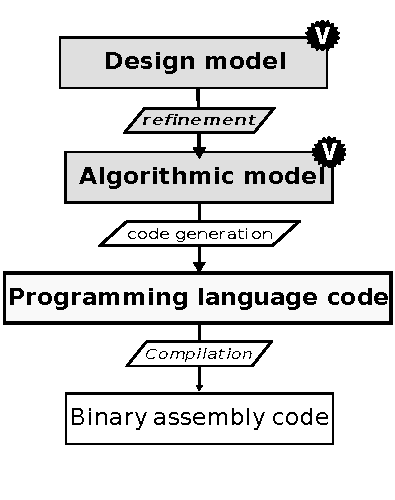
\includegraphics[height=.5\textheight]{figures/b-method-actual_new.pdf}
    \end{center}
       \begin{itemize} \item   \small{The transformation process can introduce small bugs}
       \end{itemize}
  \end{itemize}
\end{itemize}
   

	\note{ ................... }
	
\end{frame}



\begin{frame}
\frametitle{Extended Overview}  

\begin{itemize}[<+->]
  \item The B method supports the construction of safety systems
  \begin{itemize}
    \item The last year a paper [Dantas, 2008] proposed a approach to extend the formal verification
    \item One key of this approach is the formal model of the instruction set  of execution platform % of such assembly languages
      \\ \begin{center} 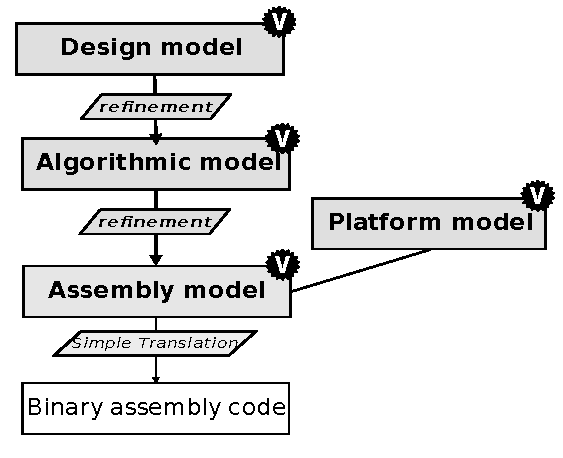
\includegraphics[height=.5\textheight]{figures/b-method-ideal_new.pdf} \end{center}
  \end{itemize}

\end{itemize}
% TO-DO Ajustar a figura

	\note{ ................... }
\end{frame}


\begin{frame}
\frametitle{Modelling Assembly Instruction Set in B}  

\begin{itemize}[<+->]
  \item The modelling is builded using some developed libraries
  \item The libraries have common concepts that can be used to others platforms of 8 or 16 bits
  \item Utilities of this formal model:
  \begin{itemize}
    \item Documentation
    \item Simulation
    \item The formal verification until the assembly level
    \item A possible support to verify the Z80 design

  \end{itemize}
\end{itemize}

	\note{ ................... }
\end{frame}



\begin{frame}
\frametitle{Objective}  

\begin{itemize}[<+->]
  \item The main actual objective is represent the assembly instruction set
    \begin{itemize}
    \item The aspects no-functional are not represented: logic circuits, pipeline, data bus, \ldots 
  \end{itemize}
  \item Moreover there are many efficient ways to verify hardware

\end{itemize}
% 

	\note{ ................... }
\end{frame}



